\subsection{Quellenumwandlung}
\begin{tabular}{cccp{6cm}}
Lineare Stromquelle		& $\Longleftrightarrow$ & Lineare Spannungsquelle & Formeln \\
\raisebox{-.8\totalheight}{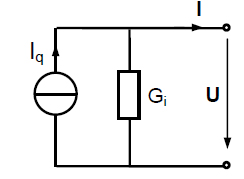
\includegraphics[width=3.5cm]{idiotenseite/images/ersatz_strom.jpg}}&
&
\raisebox{-.8\totalheight}{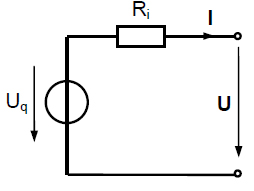
\includegraphics[width=3.5cm]{idiotenseite/images/ersatz_spannung.jpg}}
&
$I_q = \frac{U_q}{R_i} = U_q \cdot G_{i Spannungsquelle}$ \newline
$U_q = \frac{I_q}{G_i} = I_q \cdot R_{i Stromquelle}$ \newline
Der Wiederstand/Leitwert bleibt gleich \newline \\
\end{tabular}